\appendix

\section{Pre-processing Shapefiles}
\label{app:pre-processing}
Shapefiles from different sources are likely to be incompatible. In our case, the NHS CCG shapefile is incompatible with the river shapefiles. The major reason for the incompatibility is the coordinate reference system (CRS). The CRS of the CCG shapefile is EPSG:27700 (OSGB36 - British National Grid). The CRS of the river shapefiles is EPSG:4326 (WGS84 - World Geodetic System). Here we provide some pre-processing steps using QGIS (version: 3.26.0-Buenos Aires) \cite{qgisWelcome} to handle the incompatibility issue and reduce shapefile size to improve performance.

\subsection{Import Shapefiles into QGIS}
We first load all three river shapefiles into QGIS \Cref{fig:import_rivers}, followed by the CCG shapefile \Cref{fig:import_ccgs}.

{
    \begin{figure}[tbh!]
        \centering
        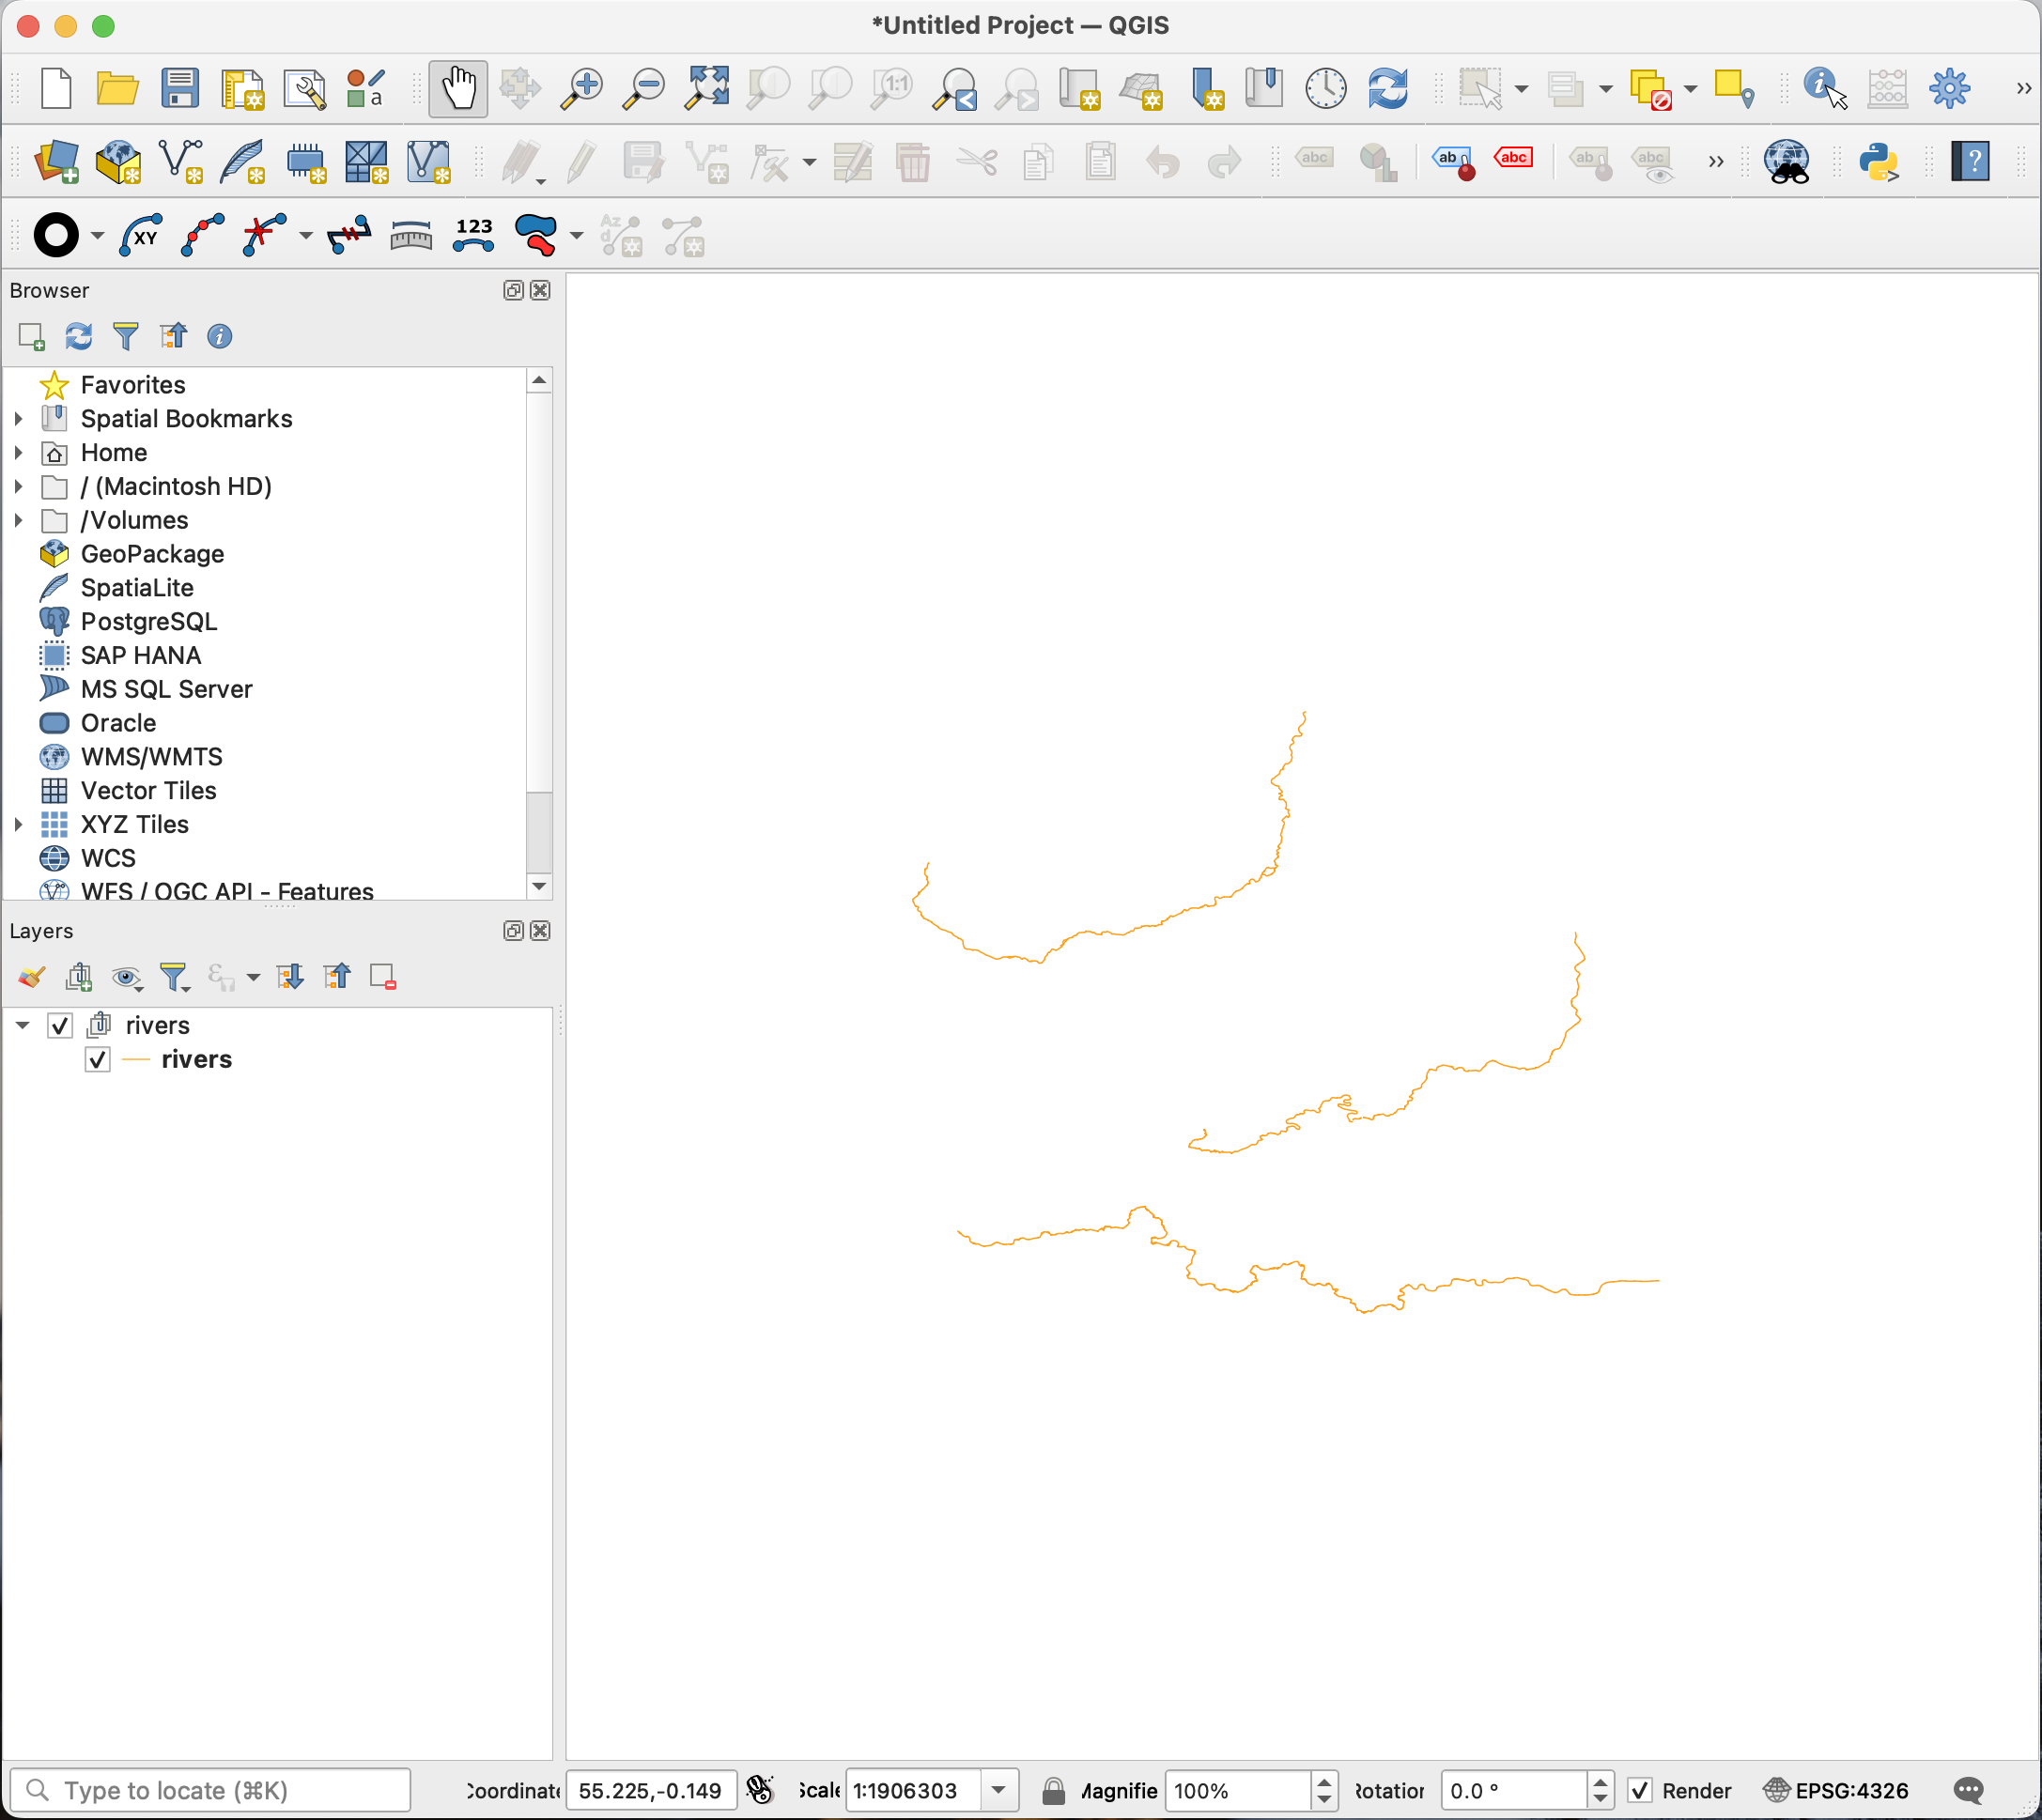
\includegraphics[width=\columnwidth]{figure/qgis/import_rivers.png}
        \caption{QGIS interface, with River Trent, River Great Ouse, and River Thames (from top to bottom) imported.}
        \label{fig:import_rivers}
    \end{figure}

    \begin{figure}[tbh!]
        \centering
        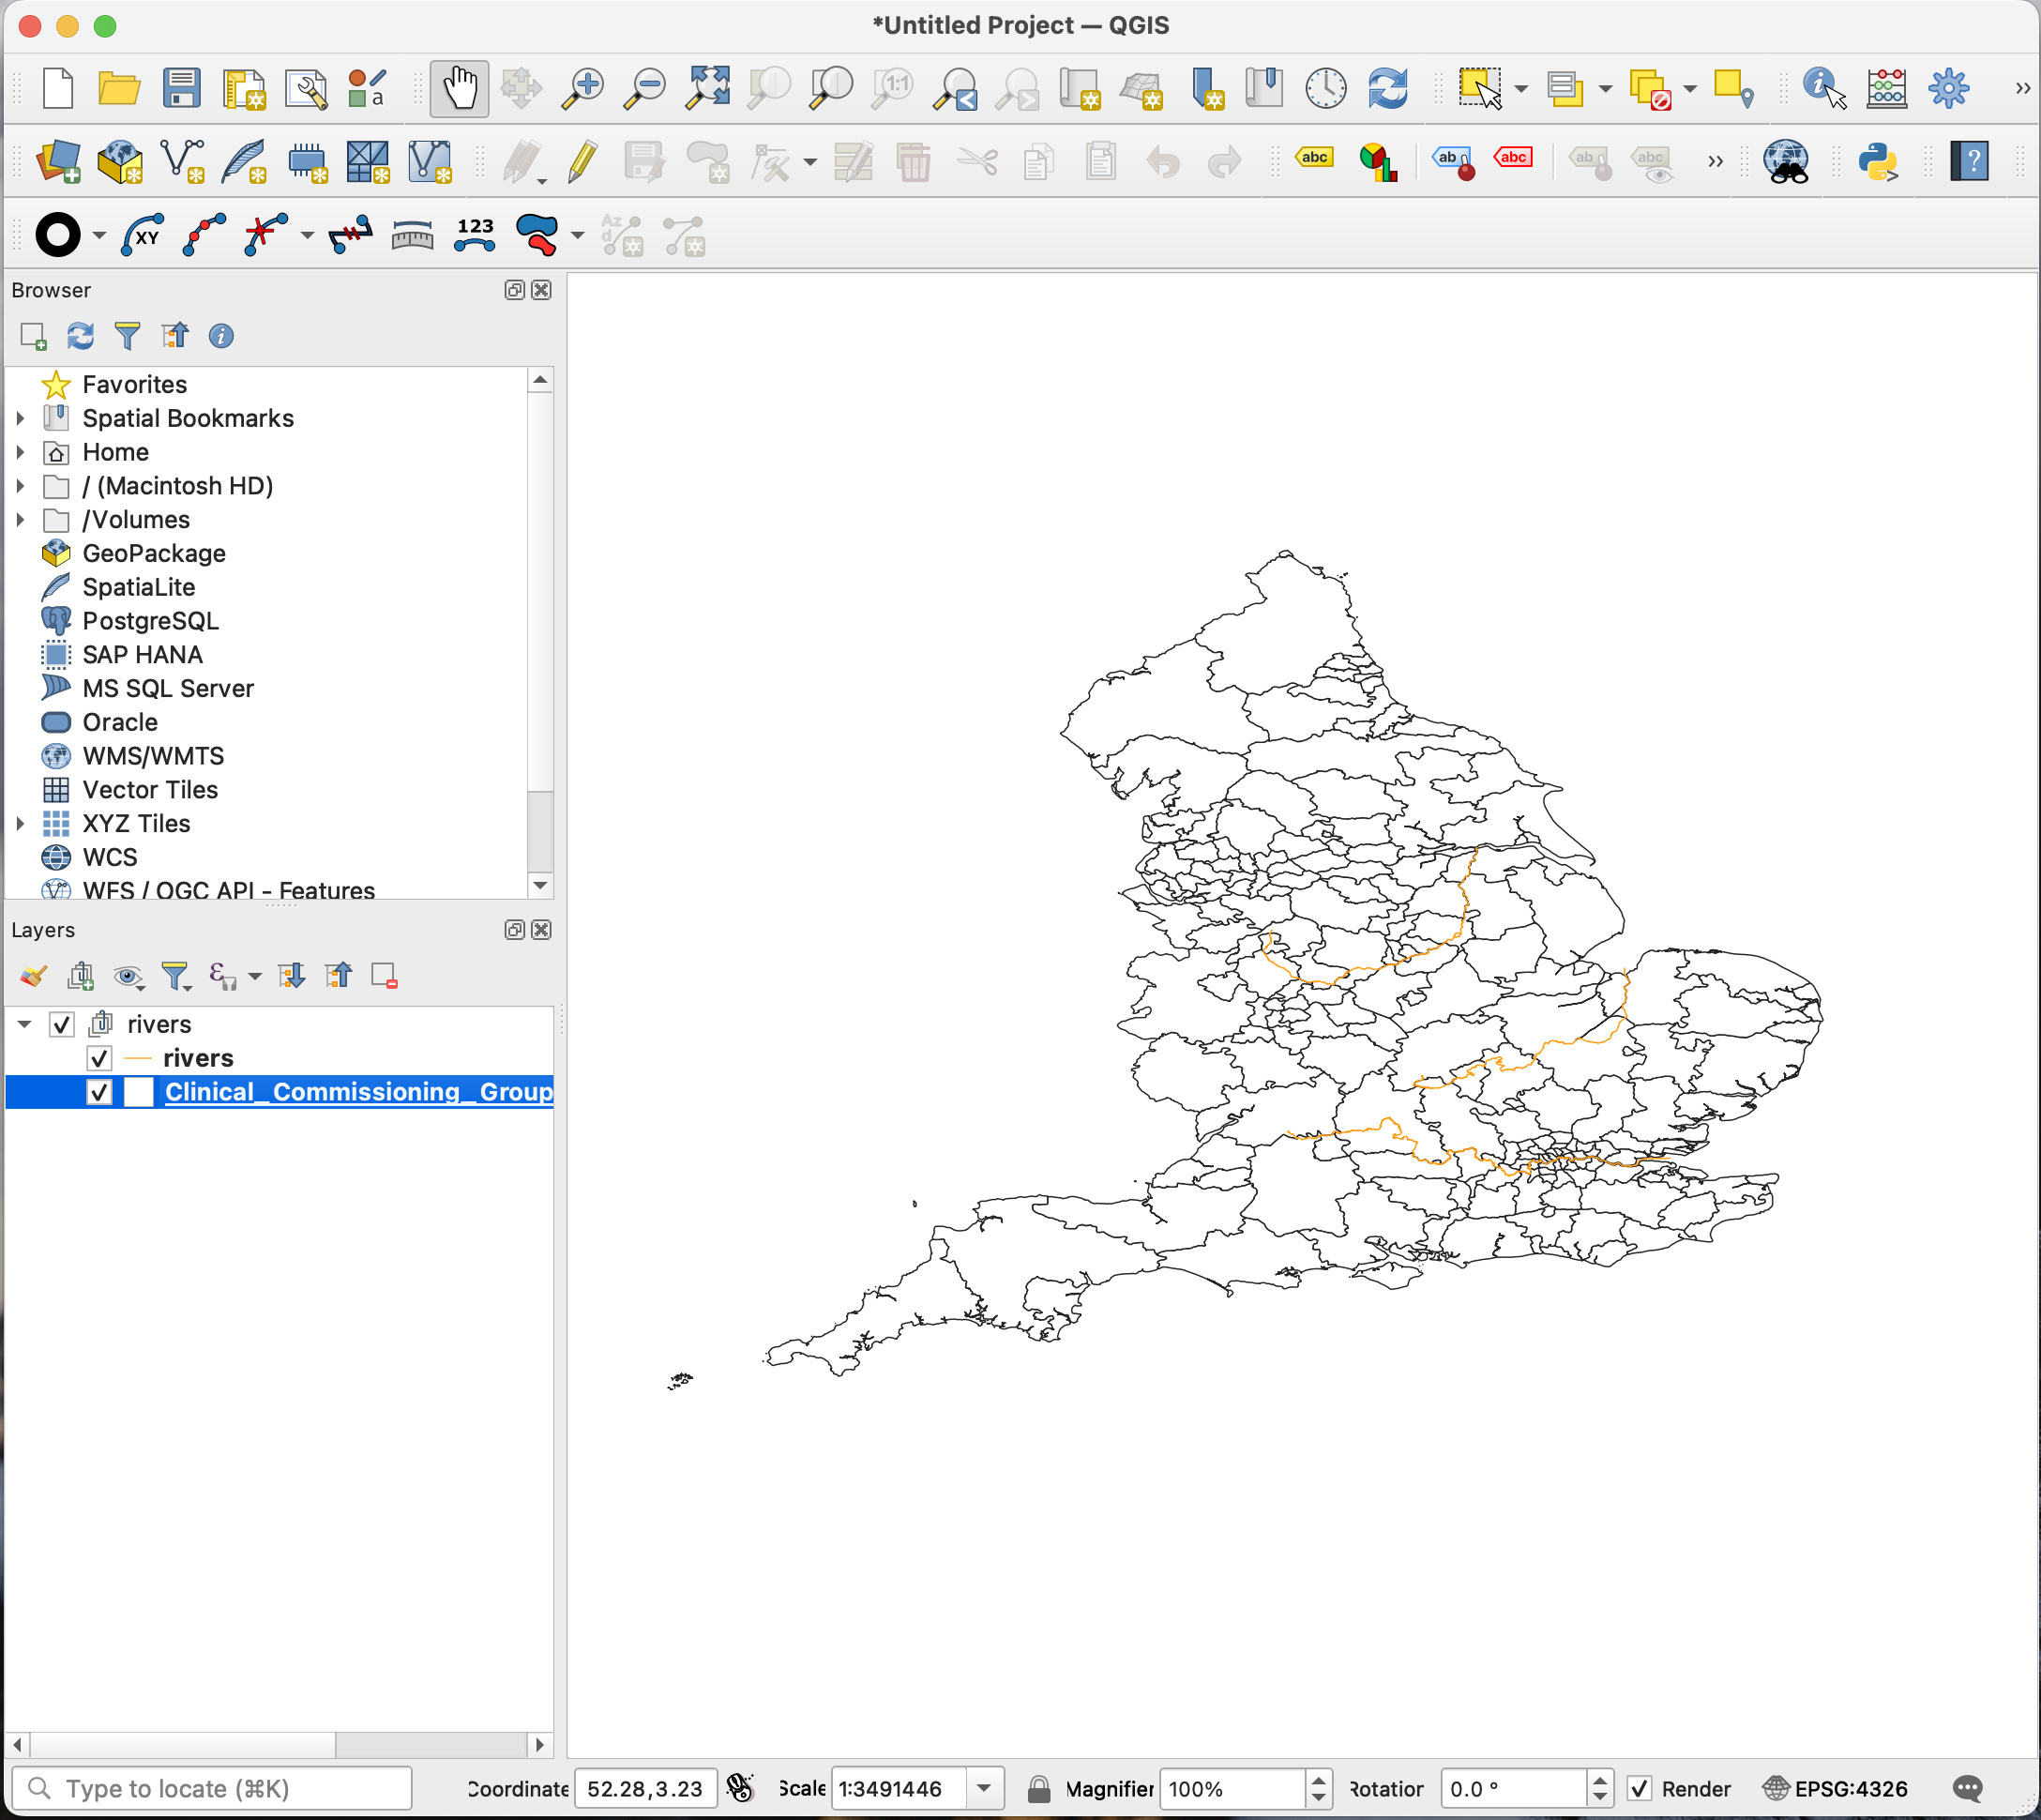
\includegraphics[width=\columnwidth]{figure/qgis/import_ccgs.png}
        \caption{QGIS interface, with all NHS CCGs imported.}
        \label{fig:import_ccgs}
    \end{figure}

    \begin{figure}[tbh!]
        \centering
        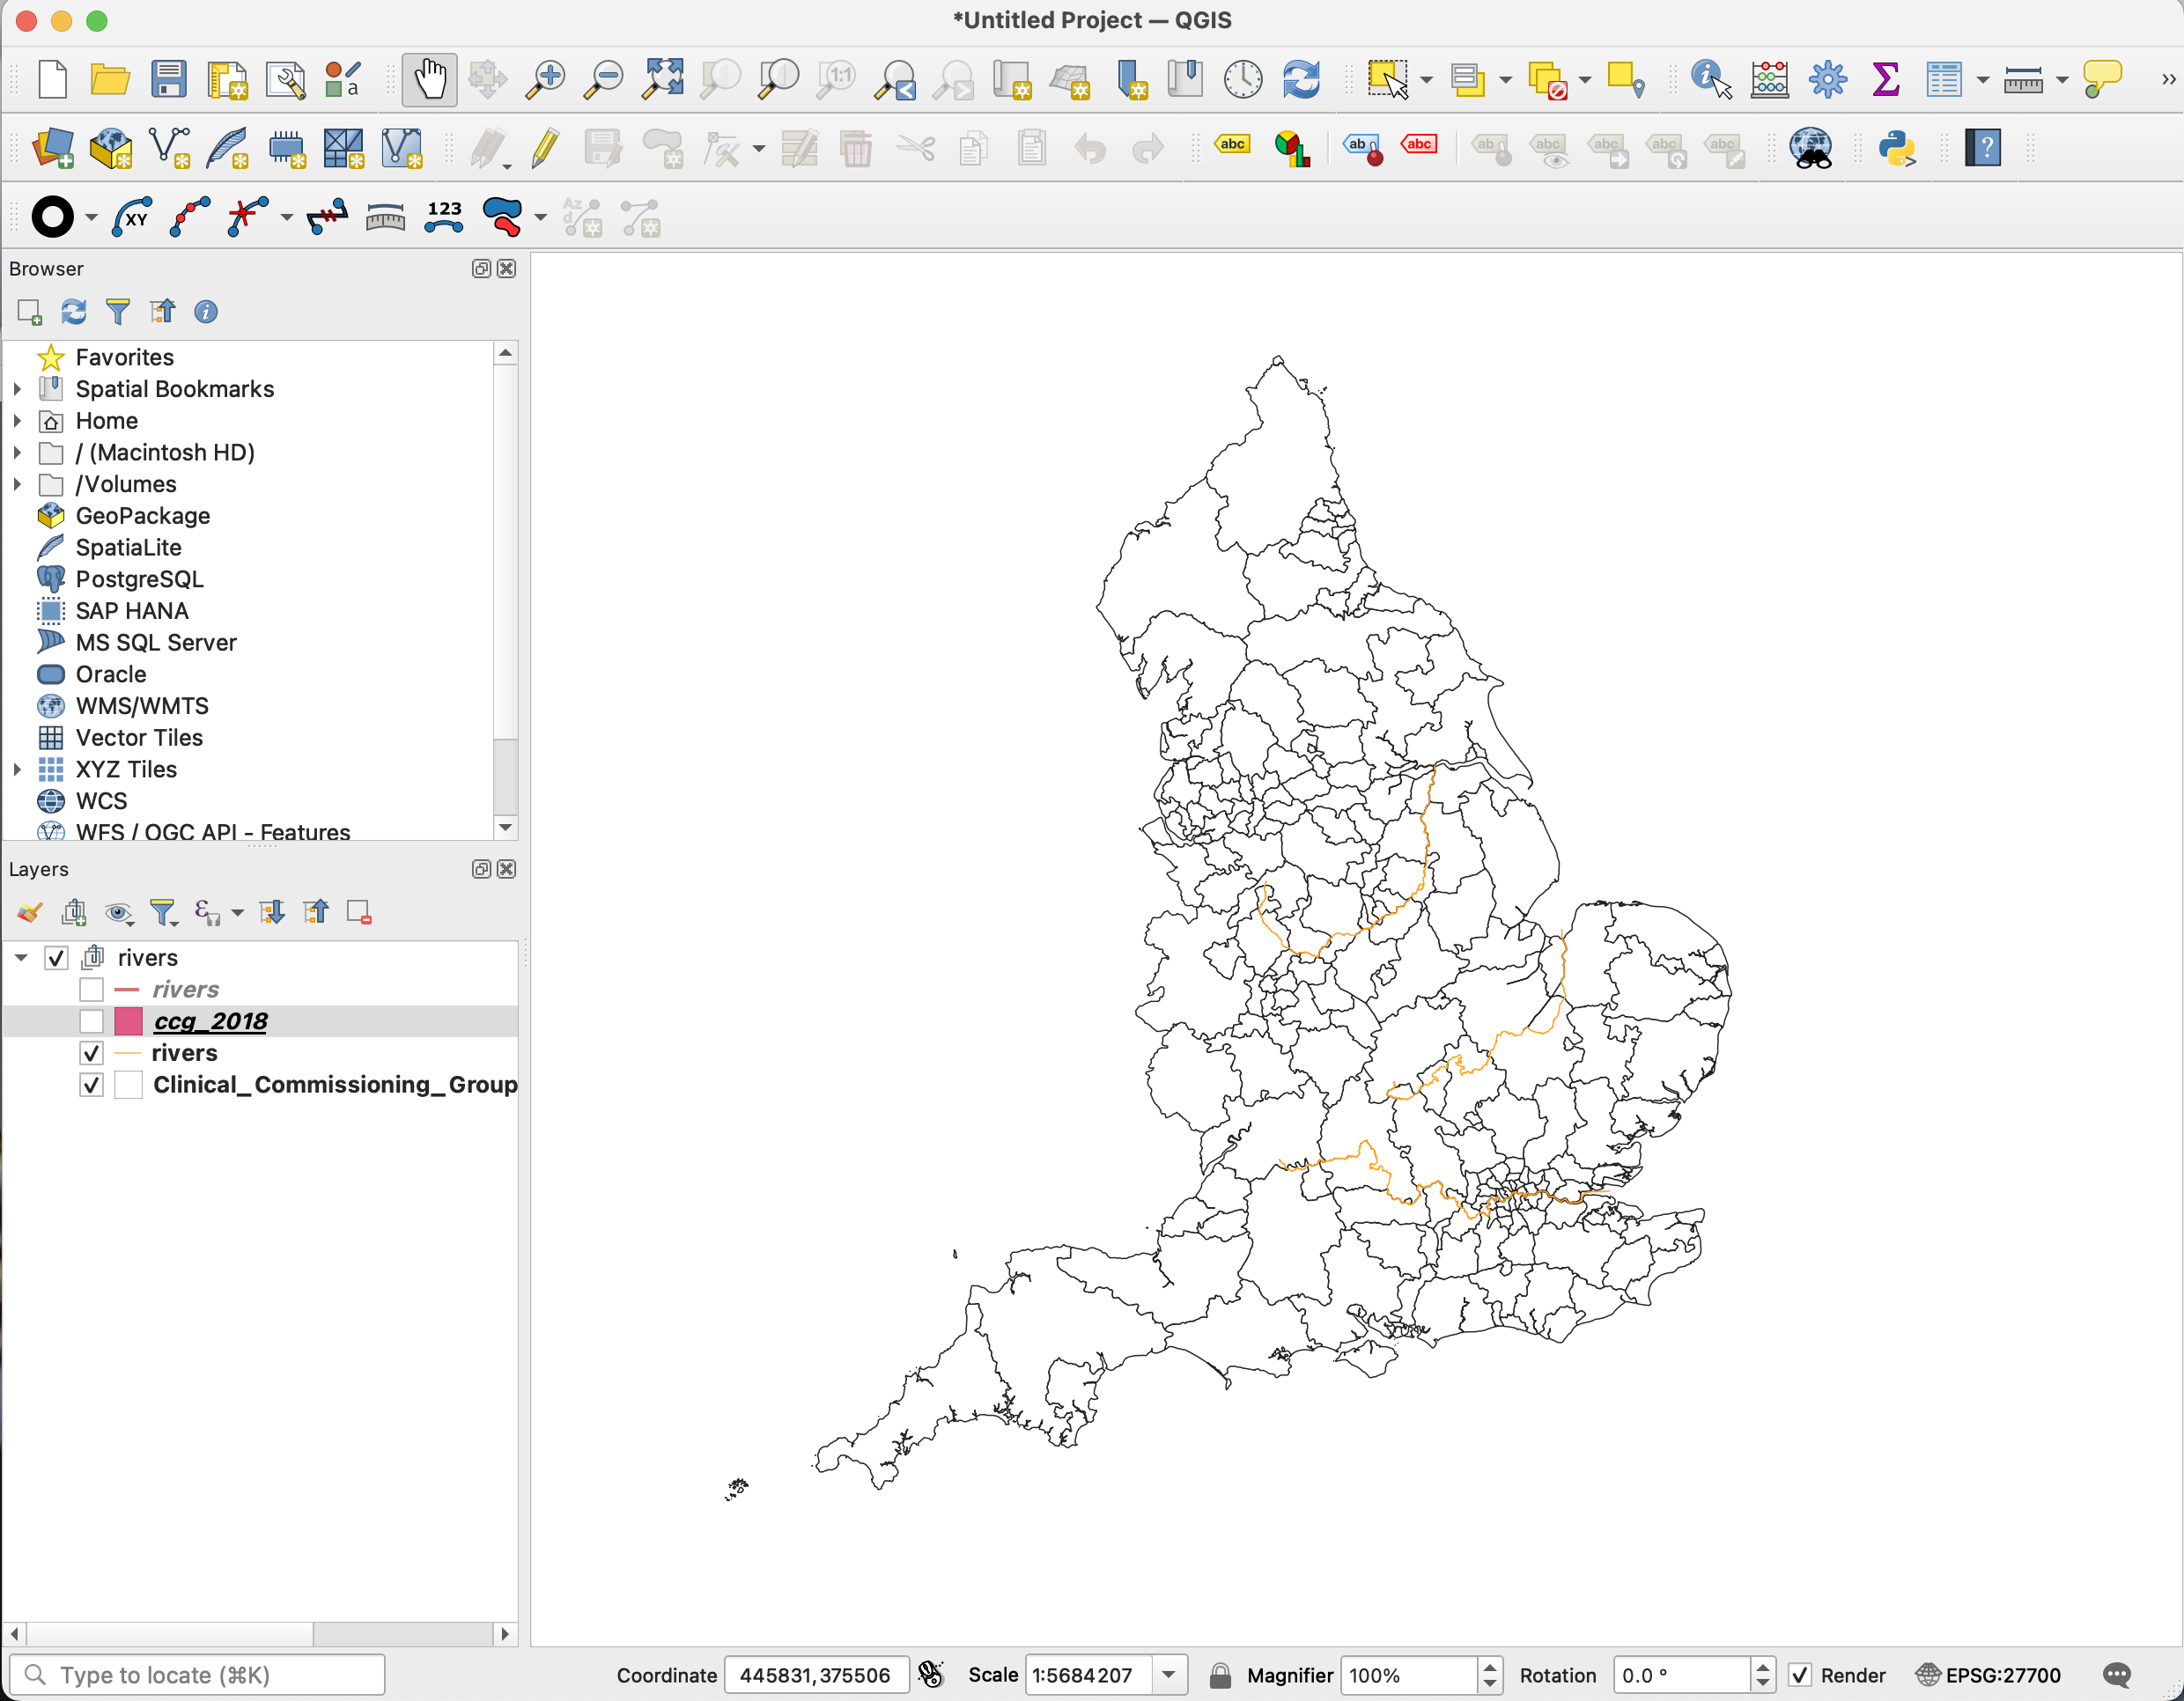
\includegraphics[width=\columnwidth]{figure/qgis/unify_crs.png}
        \caption{QGIS interface, showing the unified CRS (OSGB36) for both layers.}
        \label{fig:unify_crs}
    \end{figure}
}

\subsection{Export Shapefiles in GeoJSON and Unify the Coordinate Reference System (CRS)}

We then use QGIS to unify the CRS, and export both layers in the GeoJSON format. See \Cref{fig:export_rivers} and \Cref{fig:export_ccgs}. The unified layer is shown in \Cref{fig:unify_crs}.

{
    \begin{figure}[tbh!]
        \centering
        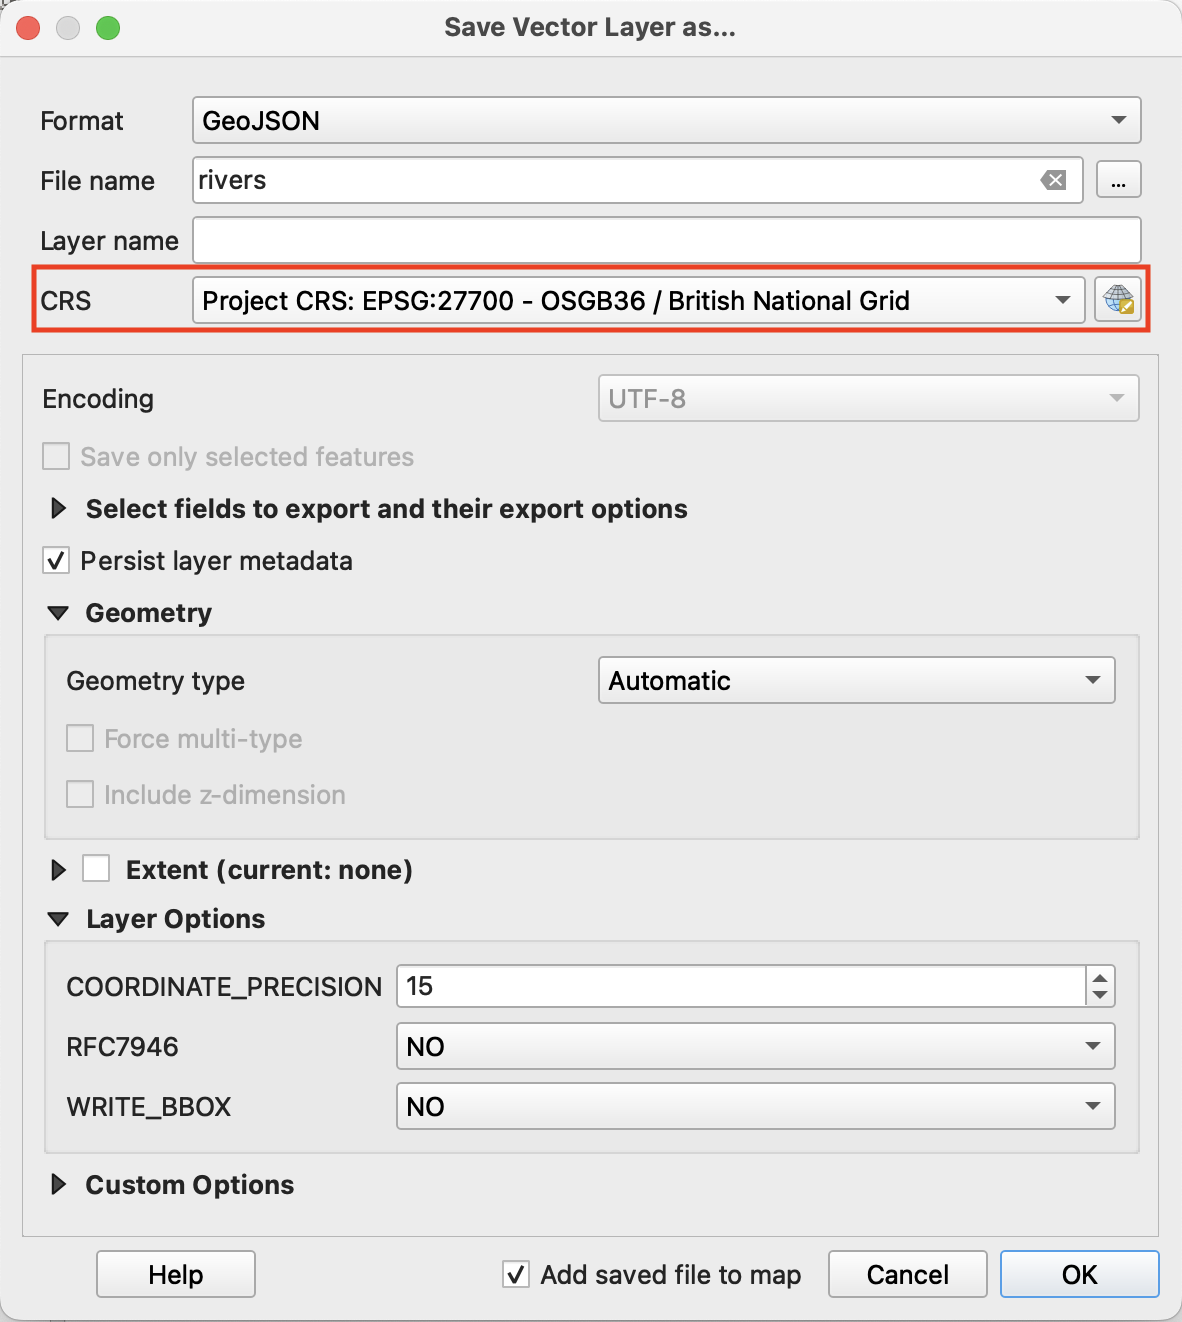
\includegraphics[width=\columnwidth]{figure/qgis/export_rivers.png}
        \caption{QGIS interface, exporting all rivers using the OSGB36 CRS in GeoJSON.}
        \label{fig:export_rivers}
    \end{figure}

    \begin{figure}[tbh!]
        \centering
        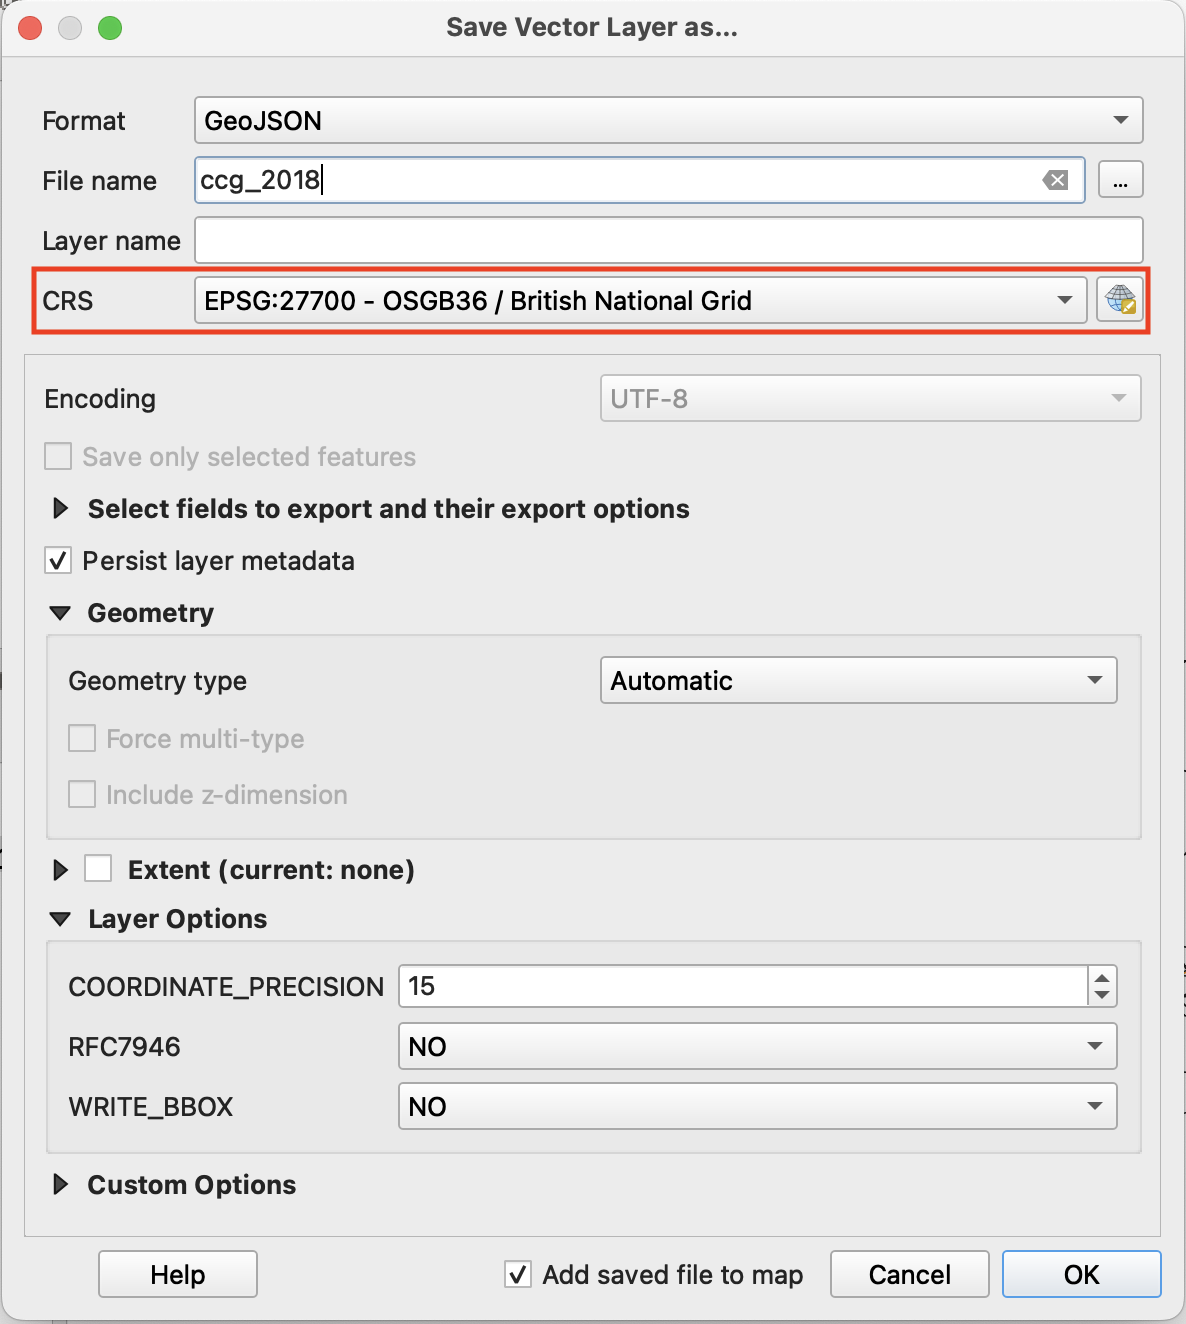
\includegraphics[width=\columnwidth]{figure/qgis/export_ccgs.png}
        \caption{QGIS interface, exporting all NHS CCGs using the OSGB36 CRS in GeoJSON.}
        \label{fig:export_ccgs}
    \end{figure}

}

\subsection{Merge Shapefiles and Reduce File Size}

We then merge two layers into one layer, and export it in the TopoJSON format using Mapshaper \cite{blochMapshaper}. Mapshaper also supports the simplification of GeoJSON shapefiles. See \Cref{fig:export_topojson}.

{
    \begin{figure}[tbh!]
        \centering
        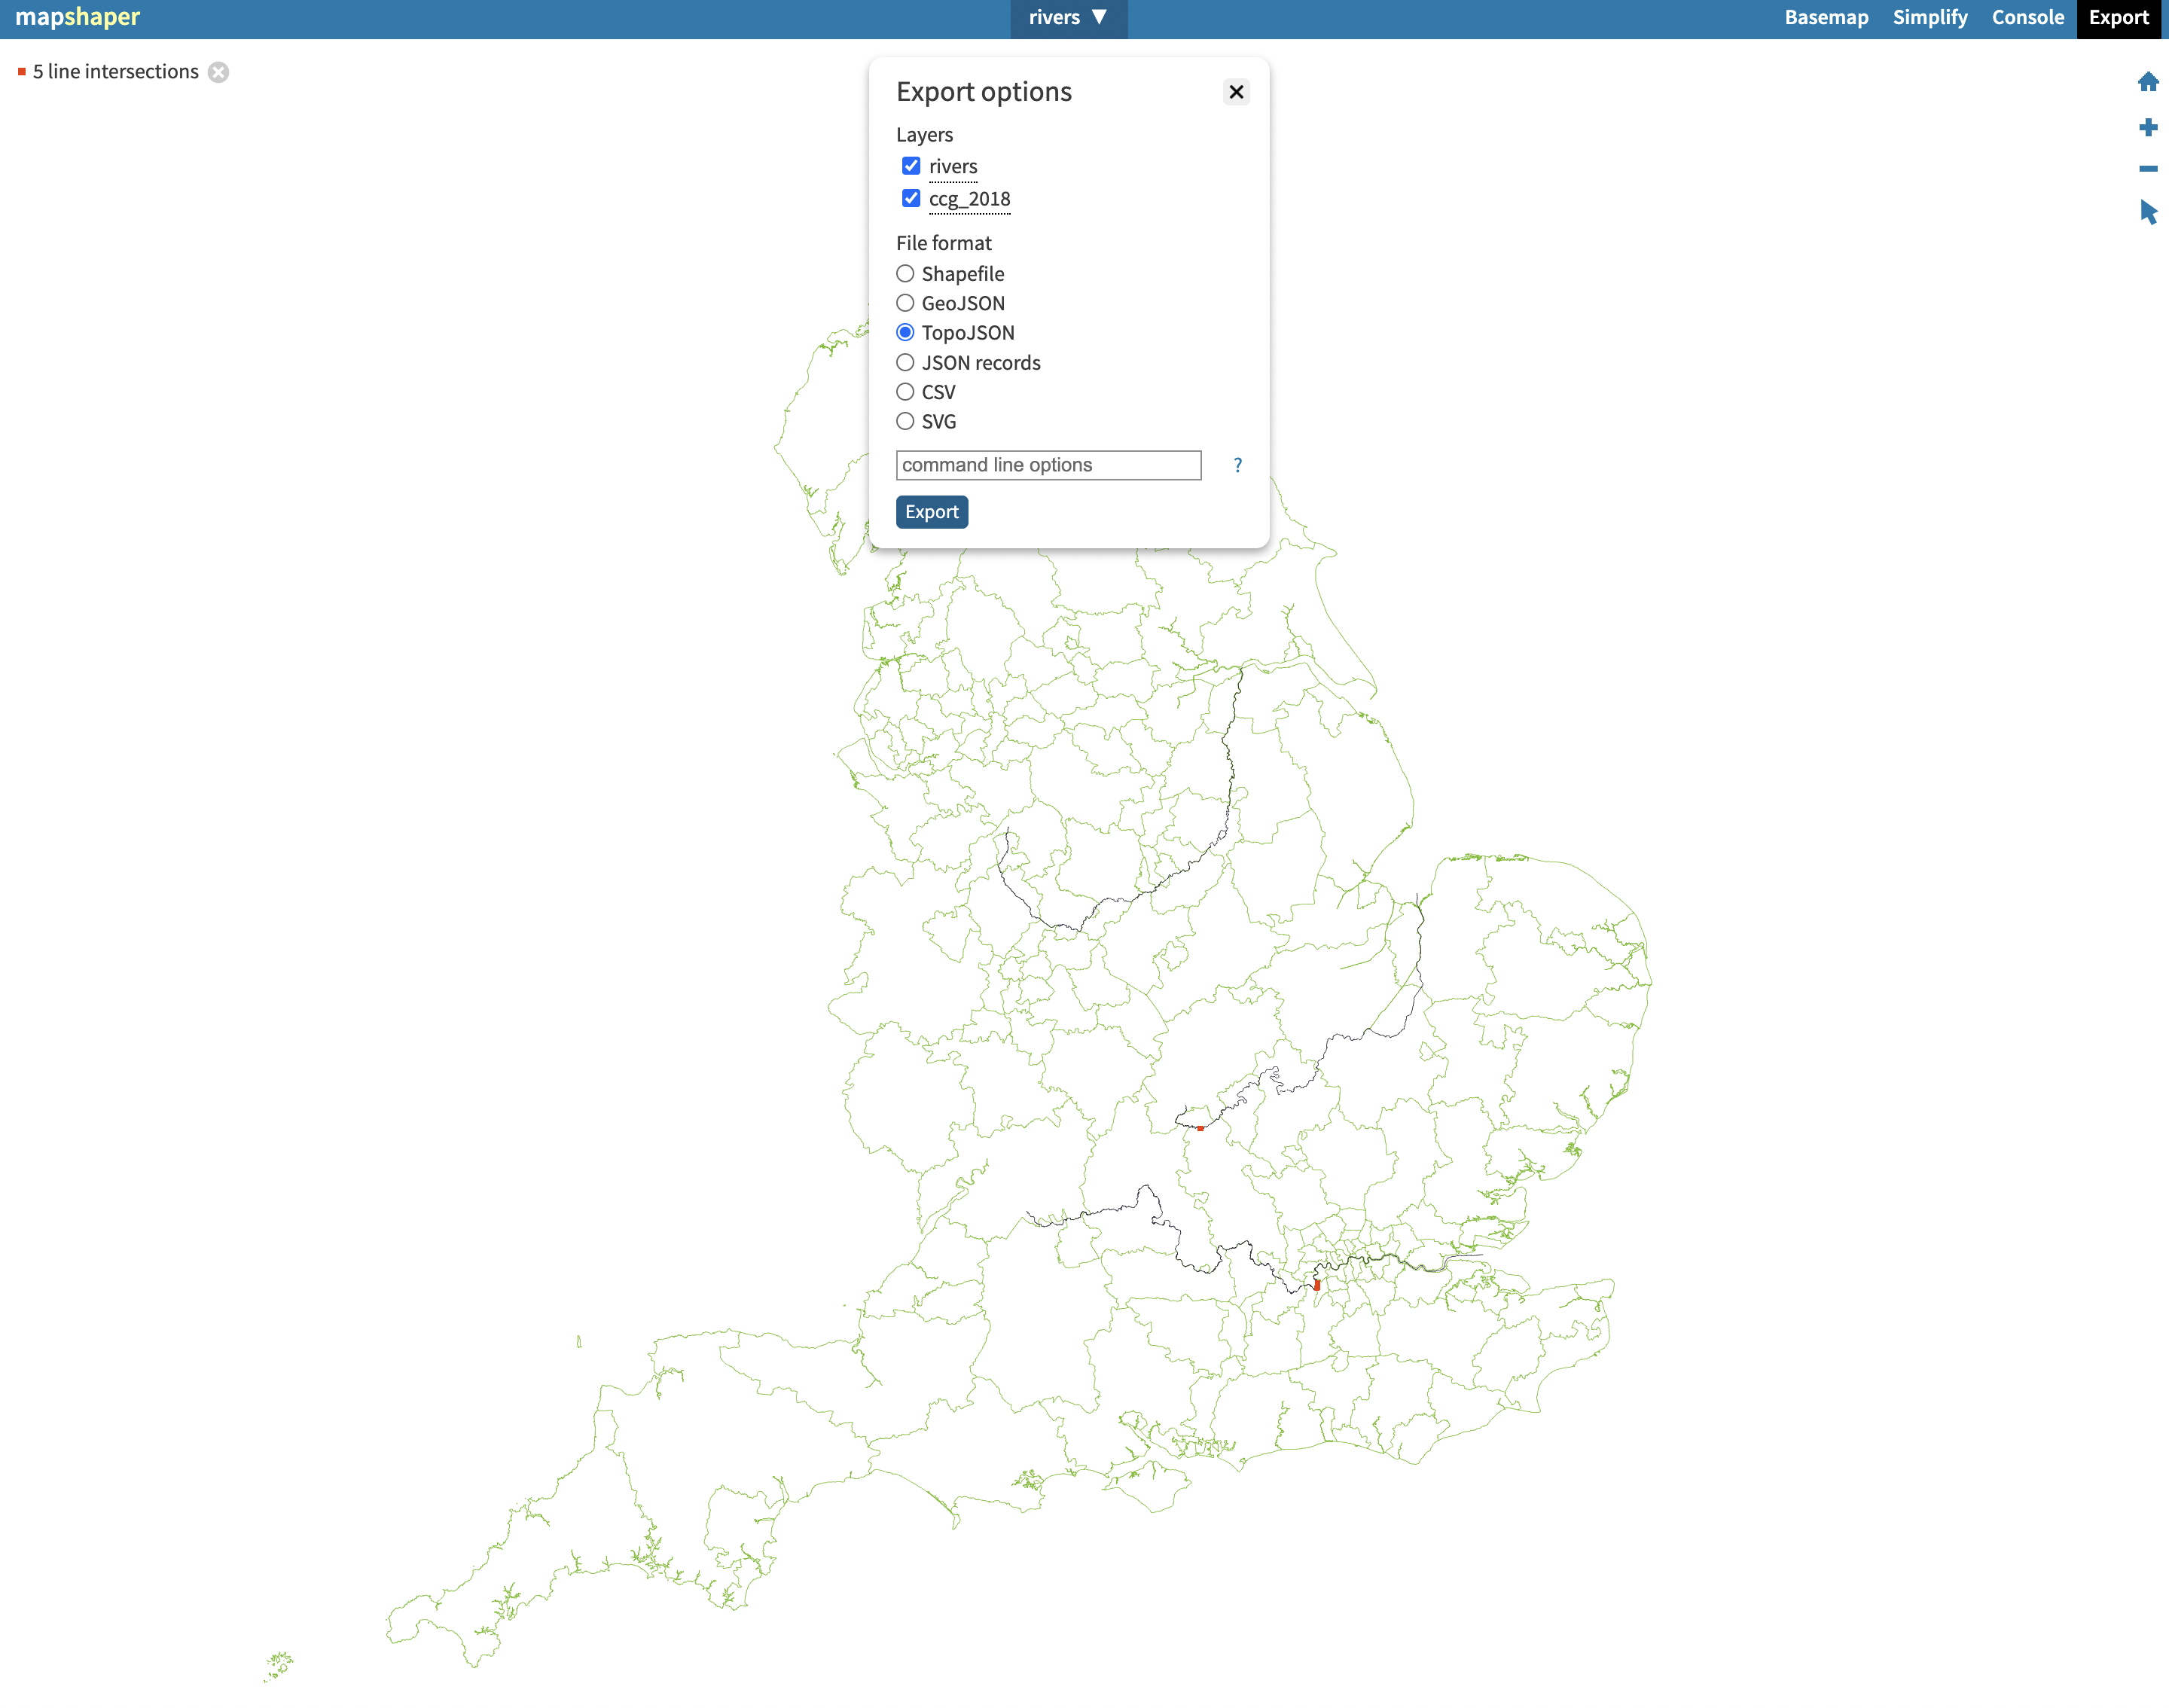
\includegraphics[width=\columnwidth]{figure/qgis/export_topojson.png}
        \caption{Mapshaper interface, merging all rivers with NHS CCGs into one layer, and export the merged layer in TopoJSON.}
        \label{fig:export_topojson}
    \end{figure}
}

\subsection{Pre-processing Result}

\Cref{table:pre-processing_result} shows the pre-processing result. The reduction in file size is significant and greatly reduces the initialization time of our implementation.

{
\renewcommand{\arraystretch}{1.5}
\begin{table}[!tb]
	\centering
	\resizebox{\columnwidth}{!}{
		\begin{tabulary}{\columnwidth}{|*{4}{l|}}
			\hhline{~|*{3}{-}}
			\multicolumn{1}{c|}{\textbf{Shapefile}} &
			\cellcolor{Mycolor2}\textbf{Original} &
			\cellcolor{Mycolor2}\textbf{GeoJSON} &
			\cellcolor{Mycolor2}\textbf{TopoJSON} \\
			\hline
			Rivers & 2.0 MB (GeoJSON) & 1.4 MB & -  \\
			\hline
			NHS CCGs & 46.6 MB (.shp, Esri vector shapefile) & 140.2 MB & -  \\
			\hline
			Merged & - & - & 16.3 MB \\
			\hline
		\end{tabulary}
	}
	\caption{The file size is reduced by 88.5\% from the original size.}
	\label{table:pre-processing_result}
\end{table}
}

\clearpage

\section{Procedure: TestIntersection}
% \begin{noindent}
    \begin{algorithm}[htb!]
        \caption{Procedure to test if a node's translation path, $ \nodeLineNV $ intersects a river.}\label{alg:check river intersection}
        \textbf{Input:} \\
        $ \nodeLineNV \gets $ the node's translation path \\
        $ \river \gets $ a river feature \\
    
        \textbf{Output:} \\
        Returns $ True $ if the node crosses a river. \\
    
        \textbf{Local variables:} \\
        $ \nodeBoundingBox, \riverEdgeBoundingBox \gets $ the bounding boxes for $ \nodeLineNV $ and $ \Edge $ \\
        $ \Edge \gets $ an edge of $ \river $ \\
    
        \begin{algorithmic}[1]
            \Procedure{TestIntersection}{$ \nodeLineNV $, $ \river $}
            
            \ForEach{$ \Edge \in \river $}
                \State $ \nodeBoundingBox \gets $ GetBoundingBox ($ \nodeLineNV $)
                \State $ \riverEdgeBoundingBox \gets $ GetBoundingBox ($ \Edge $)
    
                \If{$ \nodeBoundingBox ~intersect~ \riverEdgeBoundingBox = True $}
                    \State \Return{$ \nodeLineNV ~intersect~ \Edge $}
                    \EndIf
            \EndFor
            
            \State \Return{$ False $}
            \EndProcedure
        \end{algorithmic}
    \end{algorithm}
    %\end{noindent}
    

\section{Procedure: DerivePoint}

% \begin{noindent}

    \begin{algorithm}[tbh!]
        \caption{Procedure to derive a point based an edge and a distance.}\label{alg:derive corridor point}
        \textbf{Input:} \\
        $ \Edge \gets $ the edge used to derive the new point \\
        $ \Distance \gets $ the distance between $ \PointP $ and $ \EdgeStart $ \\

        \textbf{Output:} \\
        A point, $ \PointP $, that is distance $ \Distance $ away from $ \EdgeStart $. \\
    
        \textbf{Local variables:} \\
        $ \dx, \dy \gets $ the differences in $ x, y $ for $ \EdgeStart $ and $ \EdgeEnd $ \\
    
        \begin{algorithmic}[1]
            \Procedure{DerivePoint}{$ \Edge $, $ \Distance $}
                \State $ \dx \gets \EdgeStart.x - \EdgeEnd.x $
    
                \State $ \dy \gets \EdgeStart.y - \EdgeEnd.y $
    
                \State $ \PointP.x \gets \frac{\dx}{\sqrt{\dx^2 + \dy^2}} \cdot \Distance $
    
                \State $ \PointP.y \gets \frac{\dy}{\sqrt{\dx^2 + \dy^2}} \cdot \Distance $
    
            \State \Return{$ \PointP $}
    
            \EndProcedure
    
        \end{algorithmic}
    \end{algorithm}
    
%\end{noindent}

\section{Procedure: DeriveParallelEdge}

% \begin{noindent}

\begin{algorithm}[tbh!]
    \caption{Procedure to derive an edge, $ \EdgeParallel $, that is parallel to $ \Edge $ with a distance of $ \Distance $.}\label{alg:derive corridor edge}

    \textbf{Input:} \\
    $ \Edge \gets $ the edge used to derive the parallel edge $ \EdgeParallel $ \\
    $ \Distance \gets $ the shortest distance between $ \Edge $ and $ \EdgeParallel $ \\

    \textbf{Output:} \\
    An edge, $ \EdgeParallel $, that is parallel to $ \Edge $ with a distance of $ \Distance $. \\

    \textbf{Local variables:} \\
    $ \dx, \dy \gets $ the differences in $ x, y $ for $ \EdgeStart $ and $ \EdgeEnd $ \\
    $ \Scale \gets $ the scale of $ \frac{\Distance}{\sqrt{\dx^2 + \dy^2}} $ \\

    \begin{algorithmic}[1]
        \Procedure{DeriveParallelEdge}{$ \Edge $, $ \Distance $}
            \State $ \dx \gets \EdgeStart.x - \EdgeEnd.x $

            \State $ \dy \gets \EdgeStart.y - \EdgeEnd.y $

            \State $ \Scale \gets \frac{\Distance}{\sqrt{\dx^2 + \dy^2}} $

            \State $ \EdgeParallel.start.x \gets \Scale \cdot -\dy + \EdgeStart.x $

            \State $ \EdgeParallel.start.y \gets \Scale \cdot \dx + \EdgeStart.y $

            \State $ \EdgeParallel.end.x \gets \Scale \cdot -\dy + \EdgeEnd.x $

            \State $ \EdgeParallel.end.y \gets \Scale \cdot \dx + \EdgeEnd.y $

        \State \Return{$ \EdgeParallel $}

        \EndProcedure

    \end{algorithmic}
\end{algorithm}

%\end{noindent}